\documentclass[conference]{IEEEtran}
\IEEEoverridecommandlockouts
% The preceding line is only needed to identify funding in the first footnote. If that is unneeded, please comment it out.
\usepackage{cite}
\usepackage{algorithmic}
\usepackage{graphicx}
\usepackage{textcomp}
\usepackage{xcolor}
\usepackage[utf8]{inputenc}
\usepackage{lipsum}
\usepackage{amsmath,amssymb,amsfonts}
\usepackage{wrapfig}
\usepackage{subcaption}
% \usepackage{subfig}
\usepackage{pdfpages}
\usepackage{tcolorbox}
\usepackage{float}
\usepackage{placeins}
\usepackage[font=small,labelfont=bf]{caption} 
\usepackage{fancyhdr} 
\usepackage{graphicx} 
\usepackage{lipsum}   
\usepackage{setspace}
\usepackage{booktabs} % for better table lines
\usepackage{tabularx} % To adjust table width
\usepackage{colortbl}  % For colored rows
\usepackage{array}   
\usepackage{float}
\usepackage[table,xcdraw]{xcolor} 




\def\BibTeX{{\rm B\kern-.05em{\sc i\kern-.025em b}\kern-.08em
    T\kern-.1667em\lower.7ex\hbox{E}\kern-.125emX}}
\begin{document}

% \fancypagestyle{firstpage}{
%     \fancyhf{}  % Clear default header and footer
%     \fancyhead[L]{2024 27th International Conference on Computer and Information Technology (ICCIT)\\
%     20-22 December 2024, Cox’s Bazar, Bangladesh}  % Left side header
%     % \fancyhead[R]{Page \thepage}  % Right side header with page number
% }

\title{\fontsize{18pt}{24pt}\selectfont \textbf{
Machine Learning and IoT-enabled Traffic Management System:\\
Prioritizing Emergency Vehicles and Reducing Congestion\\
}}


% \author{
%     \begin{minipage}[t]{0.32\textwidth}
%         \centering
%         \normalsize
%         Md Faudul Isla \\
%         \textit{\normalsize Computer Science and Engineering} \\
%         \normalsize Shahjalal University of Science and Technology \\
%         \normalsize Sylhet, Bangladesh \\
%         \normalsize mdfaudulislam0@gmail.com
%     \end{minipage}
%     \hspace{0.01\textwidth} % Adds a little more gap between columns
%     \begin{minipage}[t]{0.32\textwidth}
%         \centering
%         \normalsize
%         Jakir Hasan \\
%         \textit{\normalsize Computer Science and Engineering} \\
%         \normalsize Shahjalal University of Science and Technology \\
%         \normalsize Sylhet, Bangladesh \\
%         \normalsize jakirhasan718@gmail.com
%     \end{minipage}
%     \hspace{0.01\textwidth} % Adds a little more gap between columns
%     \begin{minipage}[t]{0.32\textwidth}
%         \centering
%         \normalsize
%         M. Shahidur Rahman \\
%         \textit{\normalsize Computer Science and Engineering} \\
%         \normalsize Shahjalal University of Science and Technology \\
%         \normalsize Sylhet, Bangladesh \\
%         \normalsize rahmanms@sust.edu
%     \end{minipage}
% }


\maketitle

% \thispagestyle{firstpage}


\begin{abstract}
This paper presents an IoT-enabled traffic management system that leverages custom algorithm, and YOLOv11 machine learning models for real-time detection and classification of vehicles, pedestrians, and emergency vehicles. 
Traffic congestion is a pressing issue in urban areas, particularly in developing cities like Dhaka, Bangladesh, where mixed traffic and limited road infrastructure exacerbate delays safety risks, and similar problems.
By dynamically adjusting traffic signals based on density, and emergency vehicles present, the system minimizes unnecessary wait times and prevents lane starvation. The YOLOv11 model achieved an accuracy of 91\% in detecting and classifying vehicles and pedestrians. The solution offers a scalable, cost-effective approach to improving traffic flow and road safety in congested cities like Dhaka. Preliminary results indicate a significant reduction in congestion and overall waiting times, demonstrating the system's potential to be adapted for other developing urban areas.
\end{abstract}

\begin{IEEEkeywords}
traffic control -- machine learning -- computer vision -- object detection -- urban mobility -- emergency vehicle management
\end{IEEEkeywords}

\section{Introduction}
Dhaka, the capital of Bangladesh, is mostly known for its unbearable traffic situation, which is defined by an average vehicle speed that can descend to as low as 4.8 kilometers per hour during peak hours \cite{clar:a1}. This traffic congestion creates noticeable challenges to regular travelers and emergency services, such as ambulances and fire service trucks, which need sufficient space through crowded streets. The rapid urbanization of cities, excessive infrastructure, and a lack of useful traffic-controlling strategies increase these problems day by day leading to unnecessary delays and creating risk for emergencies \cite{clar:a16}. People have to wait hour after hour unnecessarily and waste their important time and moments \cite{clar:a2}. The running traffic management process often fails to handle these difficulties causing inefficiencies that enforce the development of an intelligent, automated traffic controlling solution from a high time.  


This thought proposes a machine learning-based traffic automation system that is built up to reduce congestion in Dhaka city while prioritizing emergency vehicles on the road first to reduce the sufferings of people. Locations leverage real-time images through camera data collected from key traffic junctions across Dhaka city, including Shahbag, Polton, Motijheel, Science Lab, Panthapath, Bijoy Sarani, and the most painful situation that people have to bear in Gulistan. To grow and train our model, we gathered a total of around 3784 images from these locations using the camera, which was closely annotated to categorize 171,436 objects into three distinct categories: Regular Vehicles, Emergency Vehicles, and Pedestrians. Which will bring a minimum of discipline on the road.


The workflow of our system starts with the collection of data which is a vital method from strategically selected key junctions. High-resolution images and video streams are delicately captured using CCTV cameras to monitor traffic conditions continuously on the road. These images are then processed, and objects within them are identified and annotated \cite{clar:a3}. The annotation process embroils tagging each detected object as one of the three categories mentioned before, facilitating the training of our machine-learning model. 


To perform our traffic automation system, we employ the YOLOv11 (You Only Look Once) object detection model, which is famous for its speed and accuracy in real-time object classification \citep{clar:a4}. Once our model is trained on the annotated dataset, it is integrated into the real-time traffic monitoring system. During operation, the system processes live video streams from the CCTV cameras, using the trained professional model to detect and classify objects dynamically and accurately. The model's primary qualities include dynamic traffic signal control, starvation management, and emergency vehicle prioritization


Our proposed traffic automation system for Dhaka describes a certain solution to the city's complex traffic difficulties. By obtaining machine learning and real-time data processing, we can set a goal to raise both traffic efficiency and safety first, ultimately improving the daily commuting experience for all road users it will be easier than before..

\section{Related Work}

Traffic regulation has been a matter of the subject of wide research, especially in densely populated urban areas where congestion is a firm problem. In Dhaka city, studies have mentioned the incapacities of old traffic control processes that rely on fixed signal timing, which can't maintain real-time traffic situations and enhances congestion during peak hours on the street \cite{clar:a5}. To define these shortcomings, researchers and paper works have proposed different types of intelligent traffic management methods that fulfill modern technologies, such as machine learning, automatic processing methods, and computer vision.


One such process is the use of deep reinforcement learning (DRL) for adaptive traffic light control, which dynamically synthesizes signal timings based on real-time traffic data on the street demonstrated that DRL \cite{clar:a6}, combined with object detection algorithms like YOLO, can optimize traffic light performance by reducing delays at intersections and prioritizing high-traffic lanes first on the street \cite{clar:a15}. This approach was further improved by integrating object detection to delicately define vehicle types, monitoring the conditions on the road, and allowing for more expert traffic signal management.


For urban areas like Dhaka, where people can face a lot of difficulties and emergency vehicle delays can have life-threatening outcomes, intelligent traffic processes have been developed to prioritize emergency vehicles on the road first. Farooq et al. introduced a priority-based traffic management system that locates signal priority like ambulances and fire trucks, thereby progressing their transit times through congested areas. Likewise, Wong et al.proposed an intelligent traffic signal control system that detects emergency vehicles using deep learning and adjusts traffic signals to simplify their passage \cite{clar:a8}.


In terms of traffic monitoring, YOLO-based object detection has become a renowned process due to its speed and validity in real-time applications. Redmon et al. pioneered the use of YOLO for real-time object detection \cite{clar:a14}, which has since been applied to several traffic scenarios, including congestion detection and vehicle classification in sections to maintain the messiness on the road. Further demonstrated how YOLO can be utilized to monitor traffic in real-time, providing eventual data for intelligent traffic control methods.


Moreover, urban traffic congestion has been resolved widely, with studies focusing on Dhaka's unique traffic patterns. Provided experimental proof on how high vehicle density and insufficient infrastructure avail to daily traffic bottleneck \cite{clar:a9}s. Such research is eventual for understanding the fundamental reasons of traffic congestion and forms the foundation for developing more adulterated traffic control solutions.

\section{Methodology}
\subsection{Real-time Video Analysis}
For traffic control issues, the methodology begins with the resolution of real-time CCTV footage captured (see Fig.\ref{fig:f1}) from multiple traffic lanes on the road at a time. YOLOv11 learning model, using advanced computer vision techniques for this purpose, is employed to define individual types of vehicles, including emergency vehicles, as well as passersby. 

\begin{figure}[H]
    \centering
    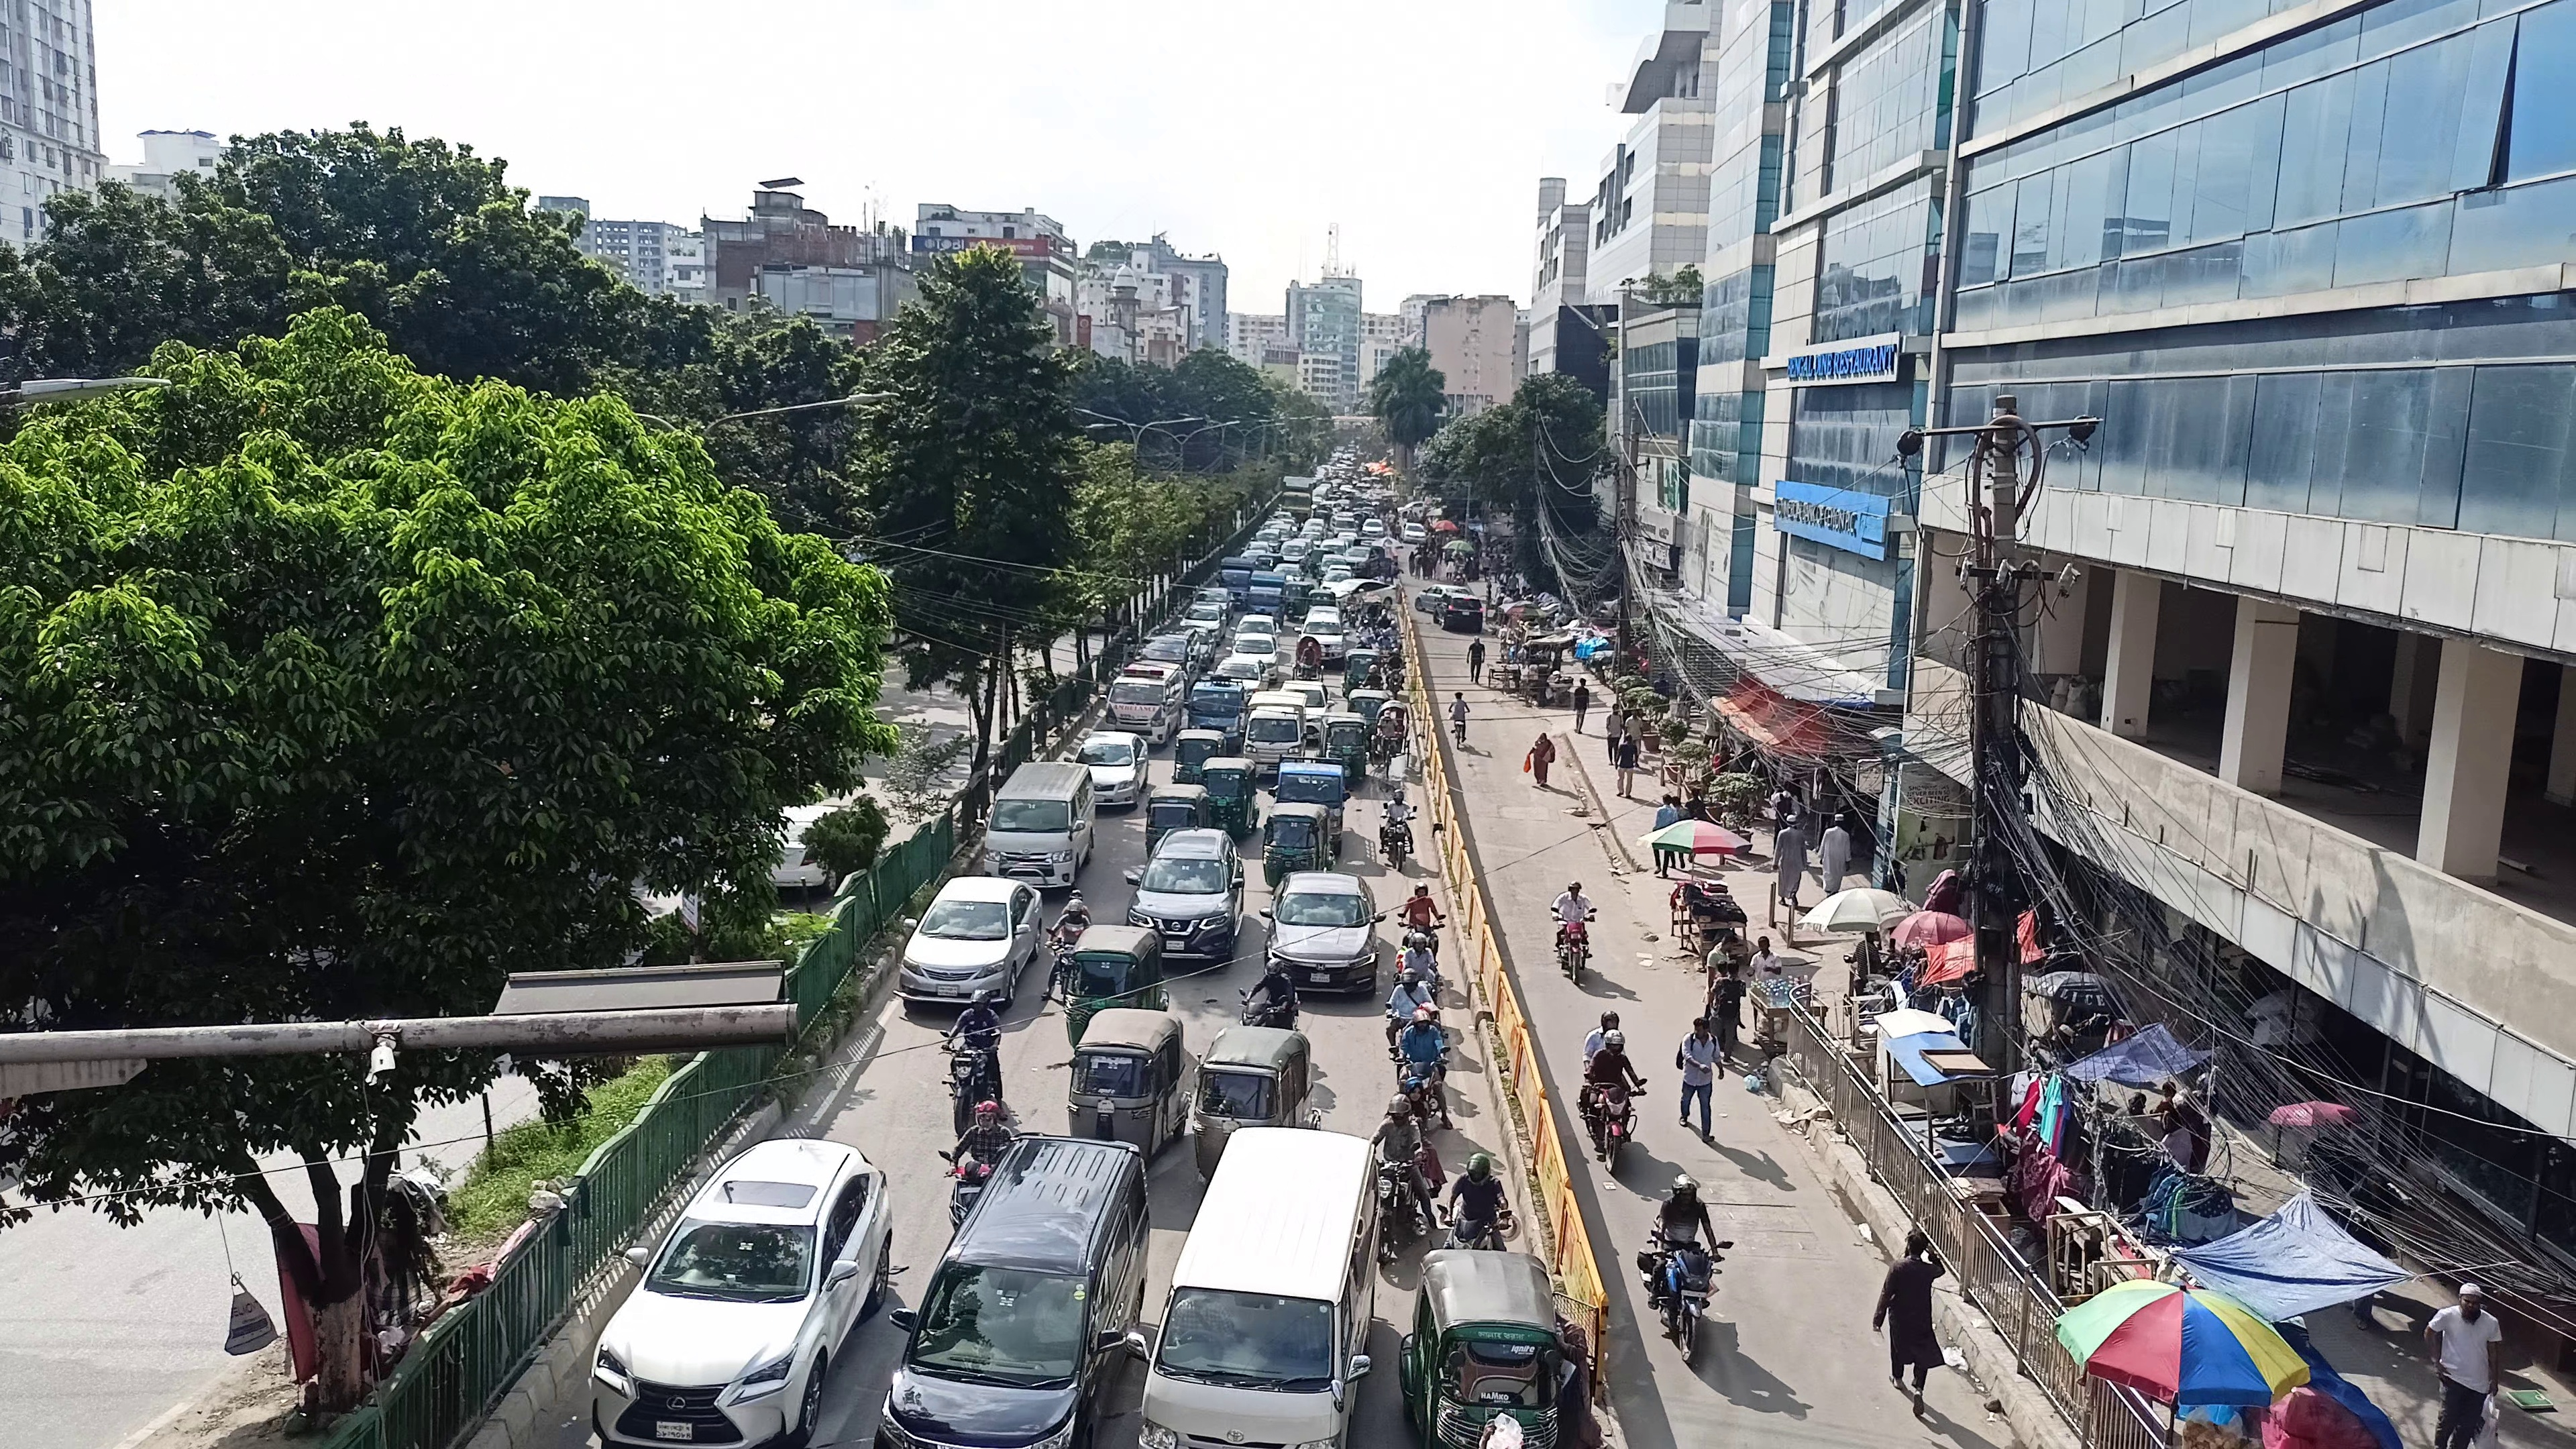
\includegraphics[width=0.5\textwidth]{7.jpg}
    \caption{CCTV footage} % Caption should work fine here
    \label{fig:f1} % Optional: Adding label for reference
\end{figure}



This experiment is performed constantly to provide updated information on traffic situations on the road in each lane, which is necessary for making rapid and proper decisions regarding traffic control. This text will wrap around the figure on the right side, making it look more integrated with the content. In this method, the real-time video experiment subsystem is designed to report adaptively to fickleness in traffic density on the road, sudden events, or violations, thereby assuring an effective traffic system. By applying neural networks, the system obtains the capacity for the conclusion, qualifying it to define and adapt to formerly unseen conditions that may arise in real-world urban traffic environments on the road.

\subsection{Object Detection}
The machine learning model is closely trained to attain a high level of exactness in identifying and classifying vehicles, emergency vehicles, and passersby (see Fig. \ref{fig:f2}). This method engages in employing state-of-the-art deep learning algorithms, including convolutional neural networks (CNNs), as well as expanding training datasets to assure strong performance under various situations. These include changes in weather (e.g., heavy rainfall, fog), illumination (e.g., nighttime versus daytime), and traffic consistency (e.g., congested versus free-flowing conditions). The training method is extensive, surrounding challenging scenarios to ensure the model's toughness and reliability. 

\begin{figure}[H]
    \centering
    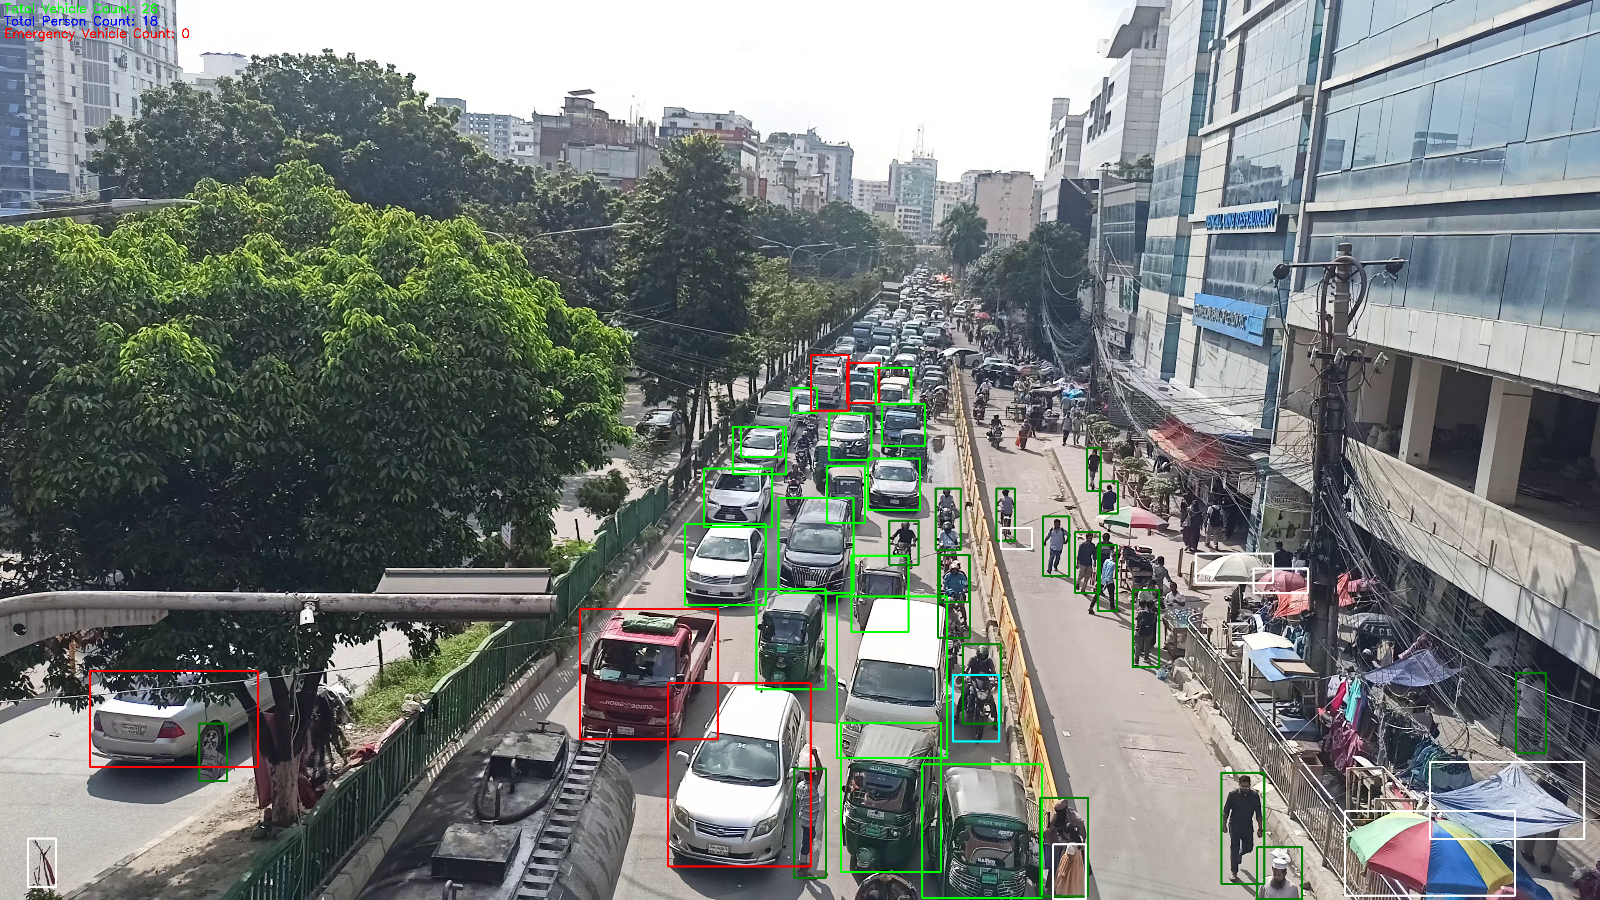
\includegraphics[width=0.5\textwidth]{8.png} % Takes the entire width of the text
    \caption{Using machine learning for vehicle and pedestrian detection.}
    \label{fig:f2}
\end{figure}
Object identification exactness is elementary to the overall proficiency and reliability of the traffic control system, as it directly influences the decision-making method. Besides, the model endures etesian retraining and optimization, assembling new data to adapt to express urban traffic situations and to improve its fateful abilities over time.

\subsection{Emergency Vehicle Handling}

Based on the identification of an emergency vehicle on the road, such as an ambulance or fire truck that needs an emergency urgent on the road, the process autonomously and immediately opens as soon as possible. The resembling traffic lane to hurry the passage of the emergency responder on the road. The method sustains the lane’s open status until the emergency vehicle has cleared every section. In those scenarios engaging multiple emergency vehicles, the process adheres to a priority-based ranking mechanism,
Assuring that each emergency vehicle on the road is benefited serially while maintaining an organized flow on the road of each vehicle. This feature is tough for reducing reaction times and is directly integrated with emergency services to improve adjustments. The method’s capability to notice different types of emergency vehicles on the road, combined with its progressive prioritization capabilities on the road, allows for optimal traffic management during troublesome conditions, Finally contributing to public safety and Their fast movement.  Additionally, by interfacing with real-time databases using technology maintained by emergency services on the road, the process can fathom the coming of emergency vehicles on which lane and preemptively optimize traffic flow to create a clear path for the people on the road and draw a relief situation on them.

\subsection{Traffic Flow Optimization}
For non-emergency traffic, the system implements a 
\textbf{*Weighted Job First (WJF)*} scheduling algorithm to determine which lane should be opened next. The WJF algorithm assigns priority weights to each lane based on factors such as the number of vehicles present, pedestrian activity (see Fig. \ref{fig:f3}), and the elapsed time since the lane was last opened. By dynamically adjusting lane priorities,
\begin{figure}[H]
    \centering
    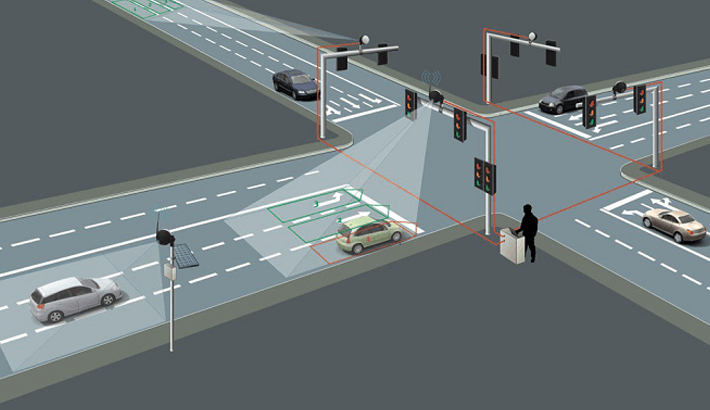
\includegraphics[width=0.5\textwidth]{2_.jpg}
    \caption{Traffic flow determination} % Caption should work fine here
    \label{fig:f3} % Optional: Adding label for reference
\end{figure}
the system minimizes congestion and ensures equitable access to all lanes, thus avoiding the risk of traffic starvation. Moreover, the system utilizes contextual data such as time of day, historical traffic patterns, and known road closures to optimize the decision-making process. For instance, during rush hours, lanes with higher vehicle densities receive greater weights to alleviate congestion. 


\subsection{Minimum and Maximum Lane Duration}
In the issue of maintaining traffic congestion, the experimental of minimum and maximum time limits for each lane's on-road open state is a tough view of the methodology. These limits are automatically adjusted based on real-time traffic situations and calculated demand. By ensuring that each lane on the road remains open for at least the minimum duration while never exceeding the maximum, the system maintains a balance between proficiency and equity in the traffic management system on the road. This approach relieves the risk of traffic buildup in less-favored lanes while assuring that high-traffic lanes take enough attention during peak periods of rush time. 
% The model also analyses fateful analytics material that leverages historical data to fine-tune lane timings on the road.
This assures optimal lane management of vehicles, reducing both the likelihood of traffic bottlenecks and the risk of enhanced waiting times for any single lane while another is starving of vehicles. The adaptive nature of this element also allows for the confirmation of passersby needs, integrating passerby crossing times into the algorithm to promote road safety for all users and travelers.

\subsection{Hardware Signal Integration}
Upon determining which lane to open or close, the system transmits a signal to the hardware controllers—typically microcontrollers (see Fig. \ref{fig:f4}) such as Arduino, Raspberry Pi, or NodeMCU—which manage the physical traffic lights. The use of resilient microcontrollers allows for precise and reliable control of traffic lights \citep{clar:a12} \citep{clar:a13}, with the added capability of scalability to multiple intersections across a city.
\begin{figure}[H]  % Adjust 0.9 for the wrapping width
    \centering
    \begin{minipage}[b]{0.16\textwidth}
        \centering
        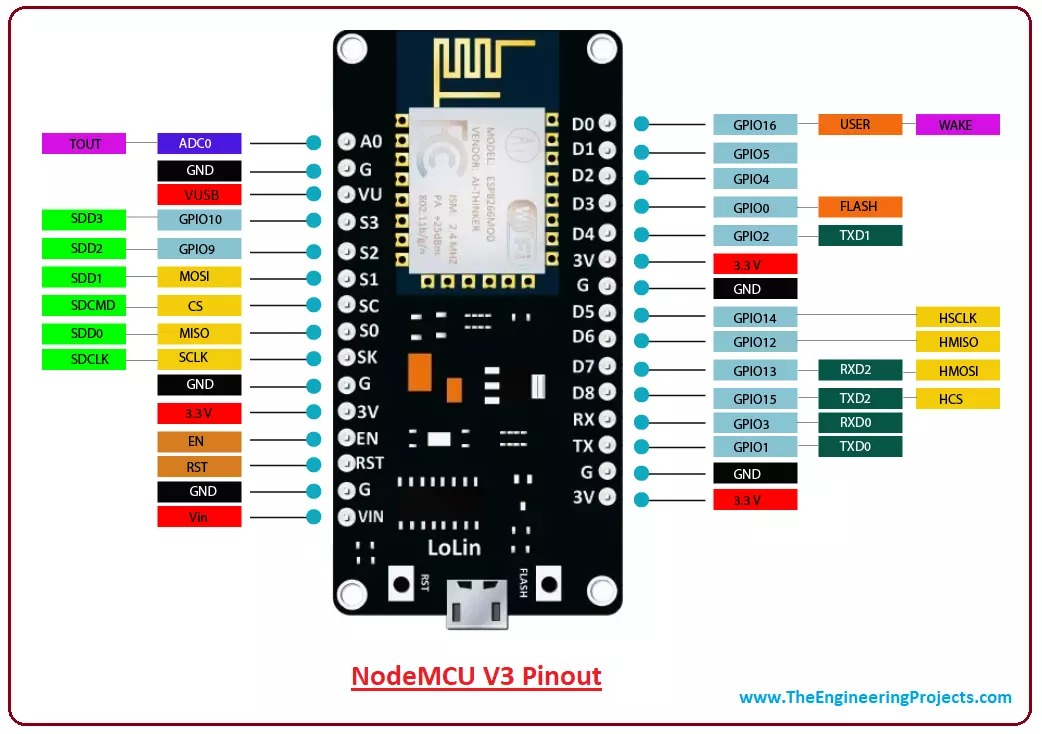
\includegraphics[width=\textwidth]{3.jpeg}
    \end{minipage}
    \hspace{0.01\textwidth} % Adds space between images
    \begin{minipage}[b]{0.16\textwidth}
        \centering
        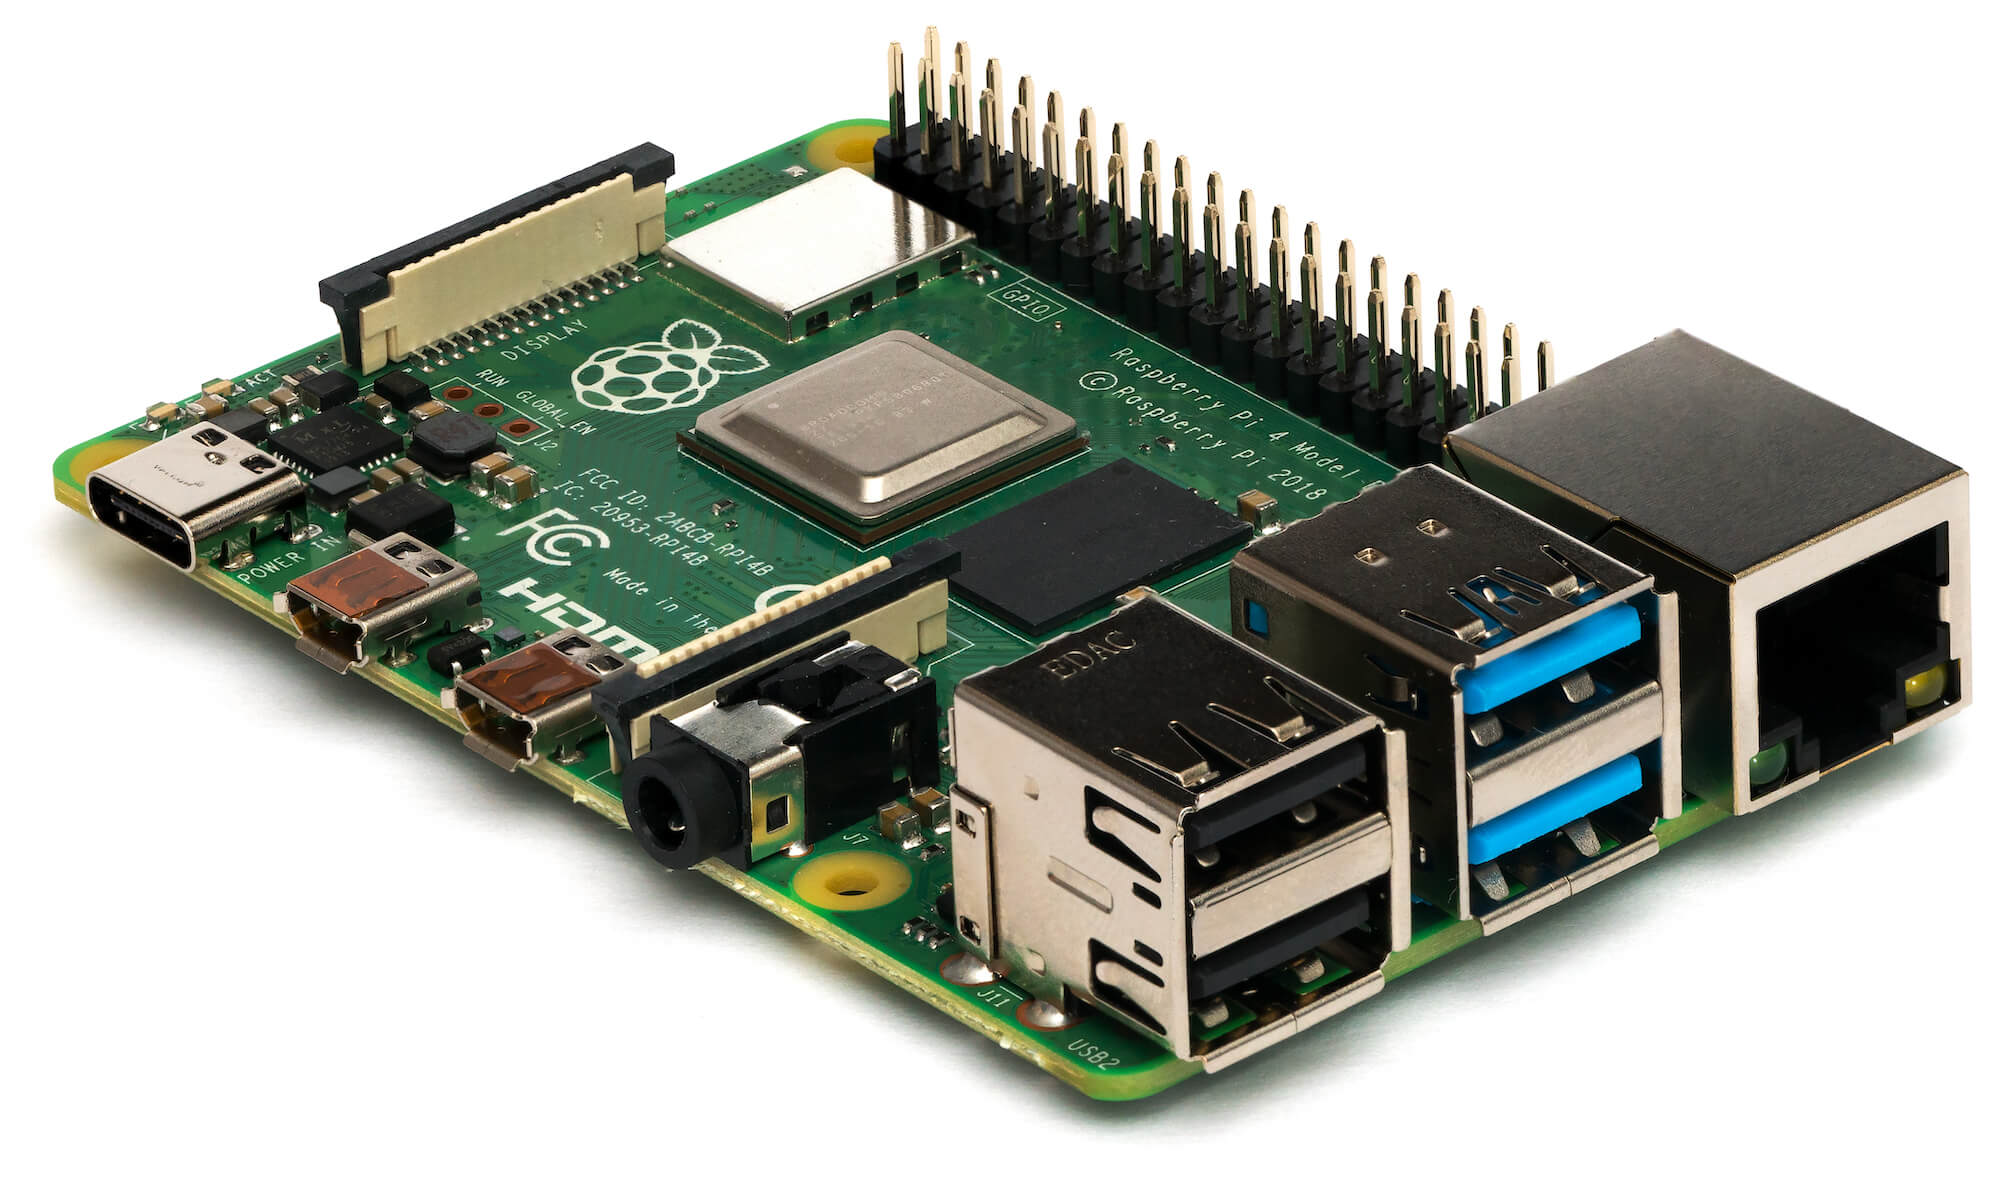
\includegraphics[width=\textwidth]{4.jpg}
    \end{minipage}
    \hspace{0.01\textwidth}
    \begin{minipage}[b]{0.16\textwidth}
        \centering
        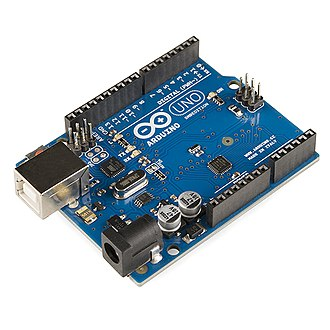
\includegraphics[width=\textwidth]{5.jpg}
    \end{minipage}
    \caption{Microcontrollers}
    \label{fig:f4}
\end{figure}
These microcontrollers serve as the interface between the machine learning control algorithms and the physical traffic signal infrastructure. This deployment of an intelligent traffic management system on a broader scale. To ensure robustness, the hardware controllers are equipped with fail-safe mechanisms to maintain proper traffic light operation even in the event of hardware or software malfunctions.


\subsection{Apply Algorithm}

The traffic control system operates within a continuous feedback loop, 
consisting of sequential stages: real-time video analysis, object detection, lane prioritization, and hardware signal activation. This continuous loop structure ensures that traffic control decisions are always informed by the most current data, thereby allowing the system to adapt to sudden changes in traffic conditions, such as accidents or surges in vehicle numbers.  algorithmic control and human expertise.
% \clearpage
% \begin{figure}
%   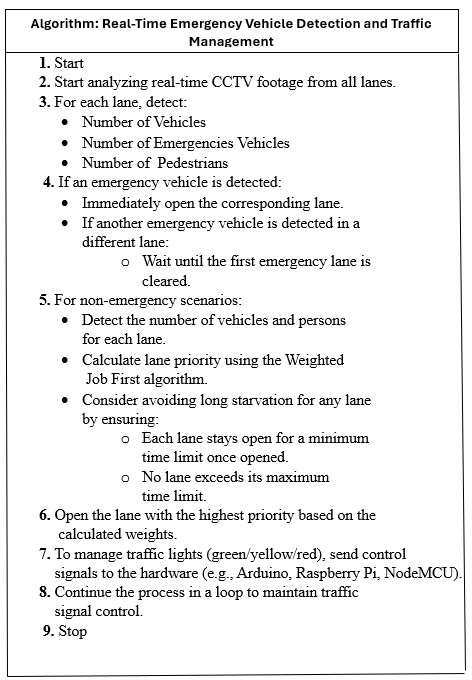
\includegraphics[width=\columnwidth]{10.png}
%   % \caption{Example of a simple single-column figure. Don't put this
%   %   too early in the document since we don't want it to go in the
%   %   first column.}
%   \label{fig:simple}
% \end{figure}
\noindent % Prevent indentation
\begin{minipage}{0.5\textwidth}
    \centering
    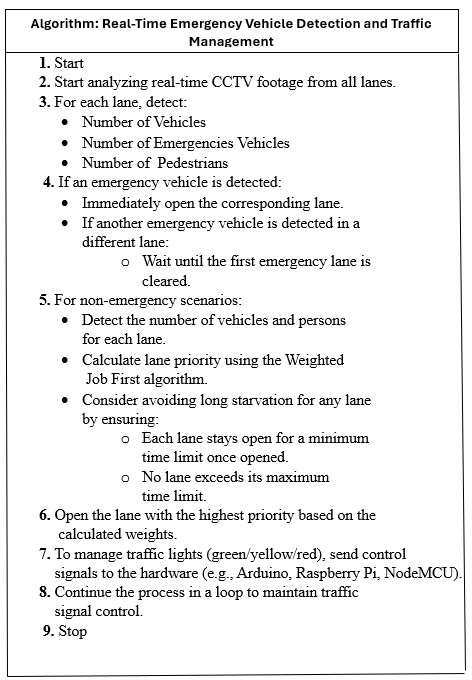
\includegraphics[width=\textwidth]{10.png} % Image takes full width of the 50% column
    \vspace{0.3cm}
    % \captionof{figure}{Pseudo Code}
\end{minipage}%

The loop operates with minimal latency, optimizing system responsiveness and ensuring real-time adaptation to dynamic traffic environments. Furthermore, an embedded feedback mechanism analyzes the outcomes of previous iterations to optimize future decision-making. This iterative learning approach facilitates continuous improvement in traffic control efficiency. If unusual patterns are detected—such as sustained congestion in a particular lane—alerts are generated for human operators, allowing for manual intervention when automated responses are insufficient. By integrating human oversight into the system's automated processes, the methodology maintains a balance between

\subsection{Signal Control}
To control the traffic congestion on the road the process can be manually stopped or paused to simplify scheduled maintenance. At the time of maintenance, all videos that were captured using camera analysis and hardware control methods were safely stopped to obstruct unrevised performances. Maintenance methodologies are structured to allow for serial-wise system updates on the road, including improvements to machine learning models and the integration of new functionalities, without being the reason for stavings to traffic flow at a time on the road. In this paper work prohibitive maintenance includes recalibrating both hardware elements and machine learning models to maintain high quality of exactness and system performance. This recalibration is typically directed during off-peak hours to minimize Breakdown to normal traffic experiments on the road.

\vspace{0.5cm}
\begin{minipage}{0.5\textwidth}
    \centering
    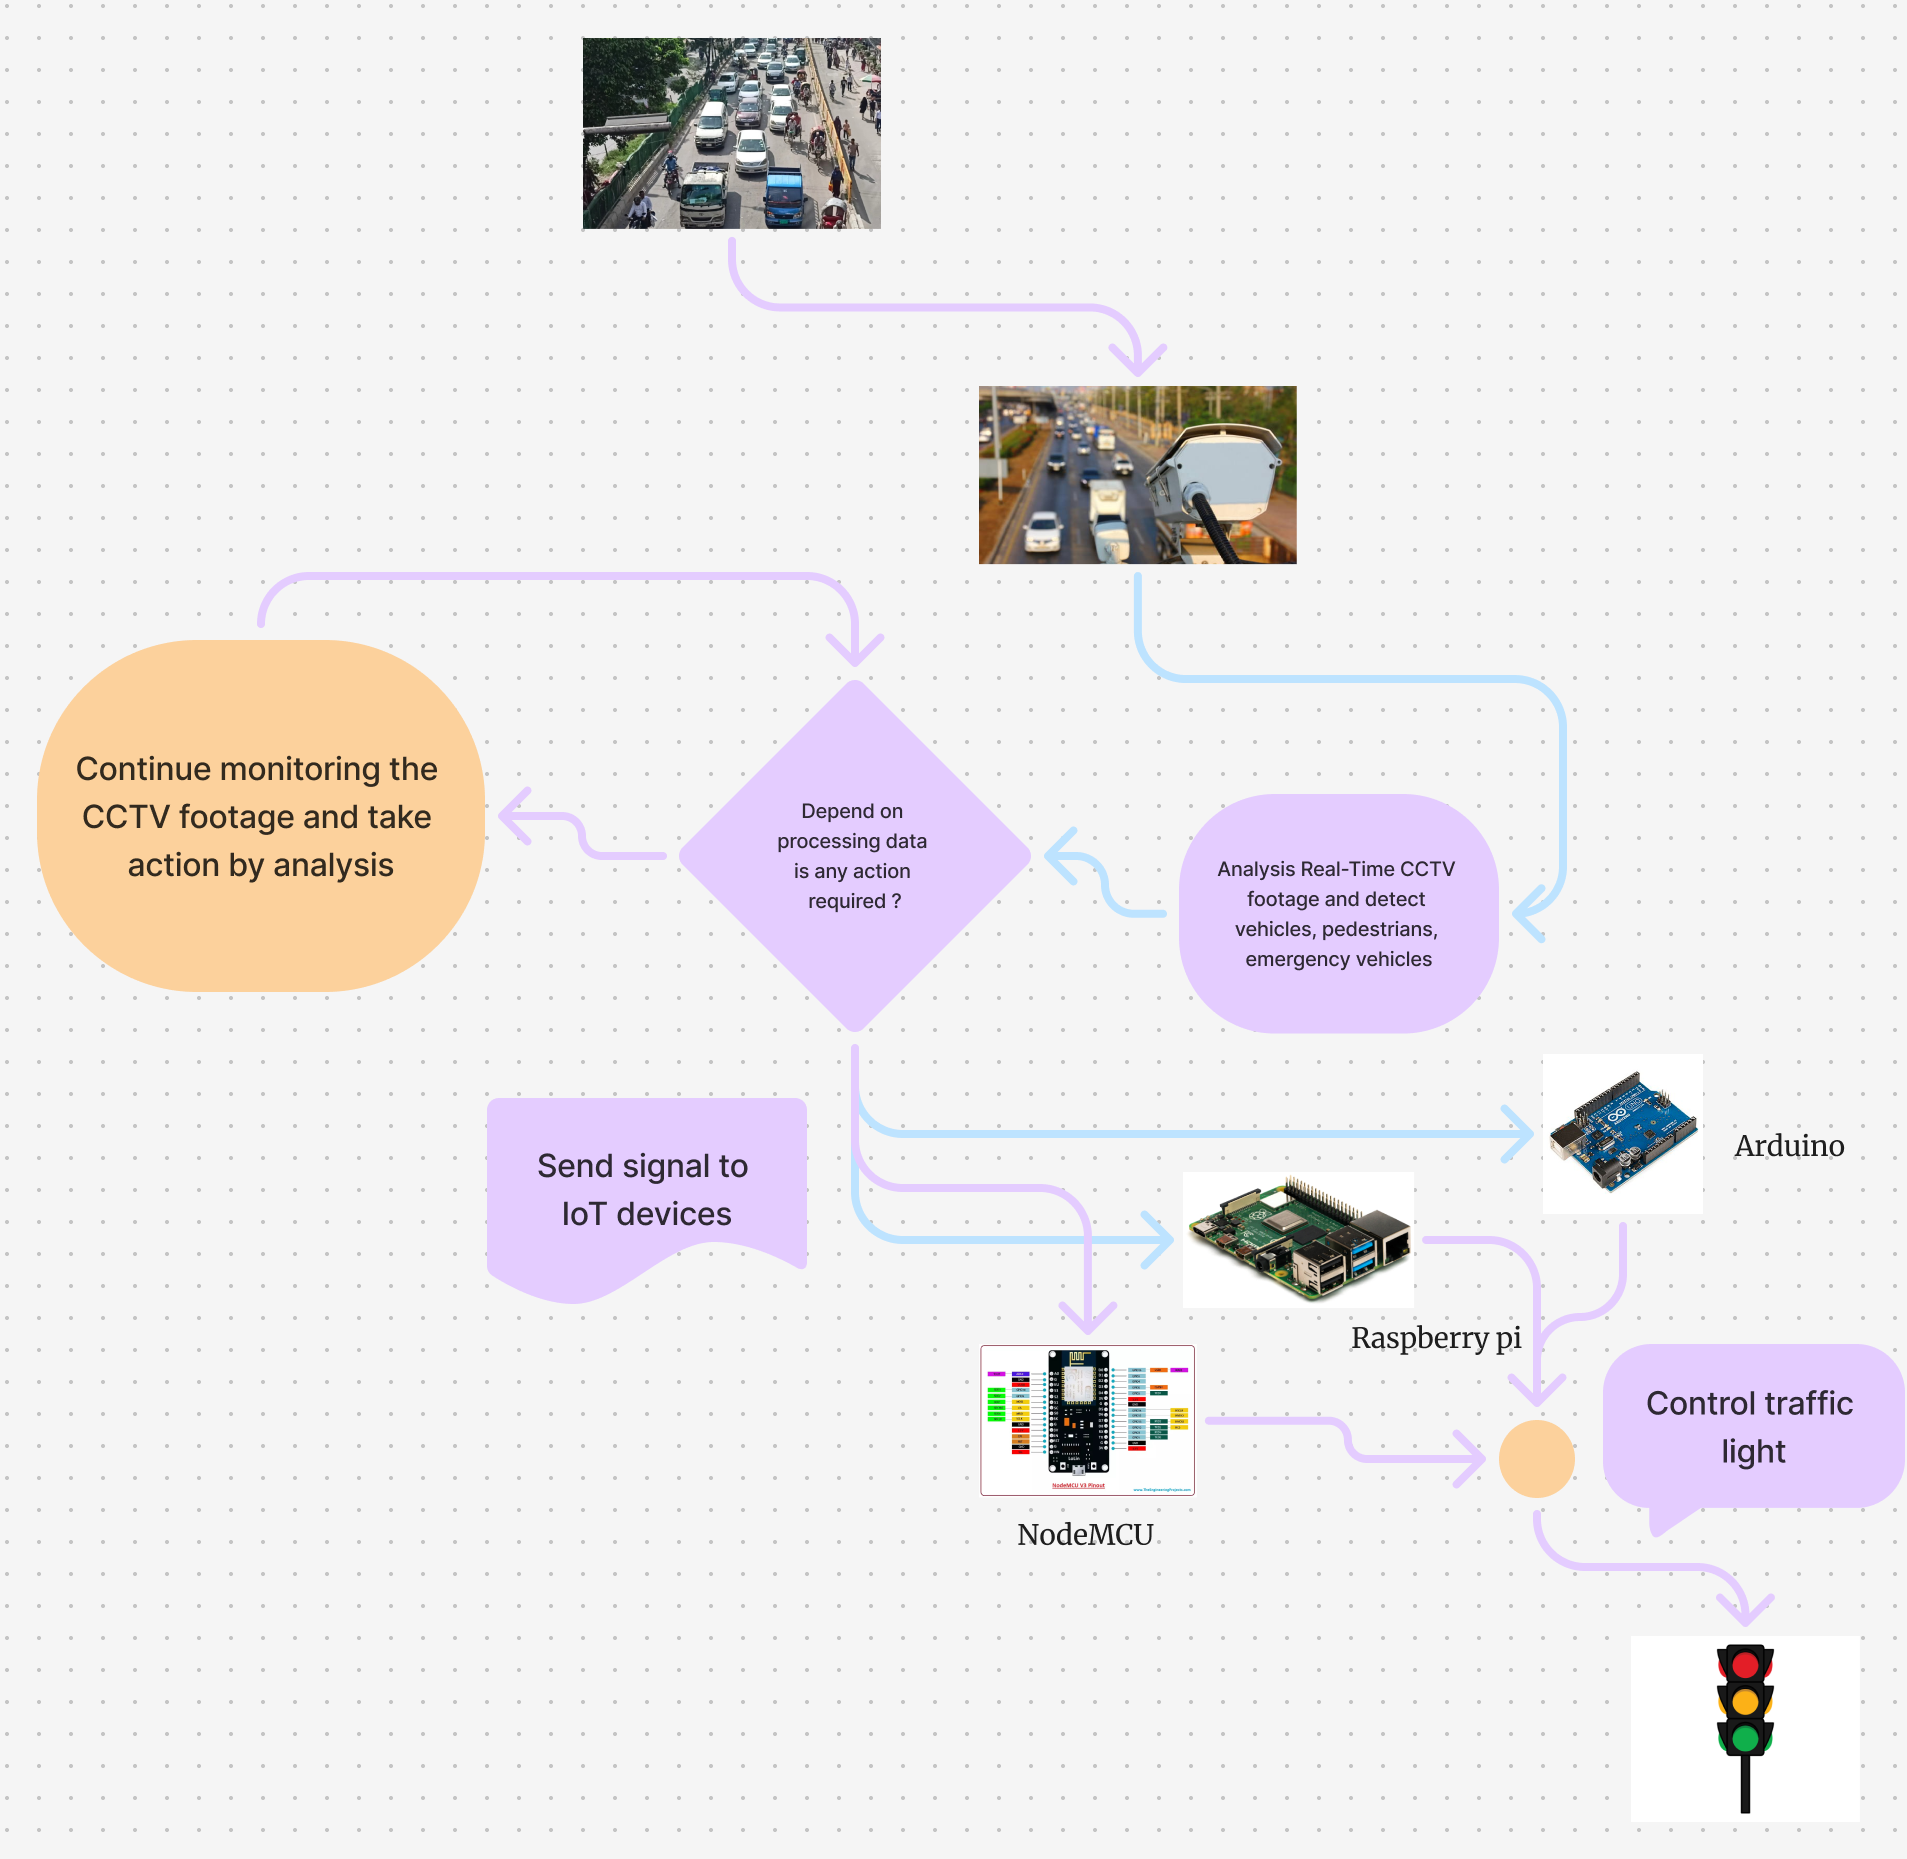
\includegraphics[width=\textwidth]{6_.png}
    \captionof{figure}{Workflow}
\end{minipage}%

Besides, automated diagnostic tools continuously count the health of both software and hardware elements, with real-time alerts created for any detected malfunctions if remain. This proactive maintenance case study not only minimizes downtime but also assures that the process operates at optimal ability at all times, maintaining the integrity and reliability of urban traffic regulation. 


\section{Result Analysis}
The project will contribute to improvements in traffic efficiency and safety. The results were collected by evaluating key metrics such as average vehicle wait time, emergency vehicle response time, decreased human interaction, and overall traffic flow consistency across multiple intersections in Dhaka and other cities in Bangladesh. We made an ML model for real-time detecting vehicles which have three class vehicles (normal vehicles), emergency vehicles (ambulance, fire truck, etc), and person. We have annotated around 107k vehicles, 63k pedestrians, and for emergency vehicles 781 (see Fig \ref{fig:f6}) and continuously adding more.

The results and confusion matrix (see Fig. \ref{fig:f7}) of our model after running \textbf{256 epochs}. We previously trained the model using \textbf{100 epochs}, \textbf{128 epochs}, and \textbf{256 epochs}, but found that running the model for \textbf{256 epochs} yielded the best results. 

% \noindent % Prevent indentation
\begin{minipage}{0.5\textwidth}
    \centering
    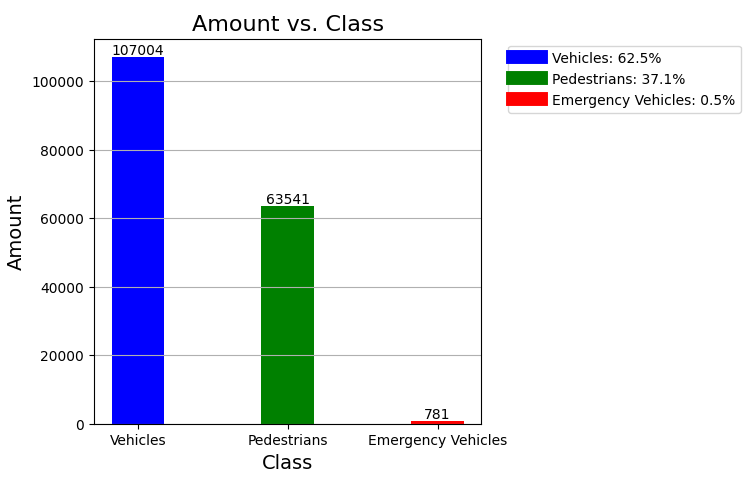
\includegraphics[width=\textwidth]{11.png} % Image takes full width of the 50% column
    \captionof{figure}{Overview of the Annotated Dataset}
    \label{fig:f6}
\end{minipage}%
\vspace{0.5cm}






The confusion matrix shows  that:
\begin{itemize}
    \item The \textbf{Emergency vehicle} class has \textbf{4 instances} that are correctly classified.
    \item The \textbf{Person} class has \textbf{2080 instances} that are correctly classified.
    \item The \textbf{Vehicle} class has \textbf{4111 instances} that are correctly classified.
    \item The \textbf{Background} class has \textbf{1222 instances} that are correctly classified.
\end{itemize}

These results demonstrate a significant improvement over earlier epochs, particularly in distinguishing between vehicles and pedestrians. The final model at 256 epochs exhibits the best performance in classifying the various traffic entities.

The chart demonstrates the distribution of bounding boxes across three categories: vehicles, pedestrians, and emergency vehicles. The model has achieved an overall accuracy of 1000 images in \textbf{79\%}, vehicle accuracy of 85\%, person accuracy of 71\%, and emergency vehicle 72\%. which shows significant progress. Also, we are working to increase it up to 99\% or more overall.  Here's a breakdown of the observations based on the data:
\begin{figure}
    \centering
    \begin{minipage}{0.5\textwidth}
        \centering
        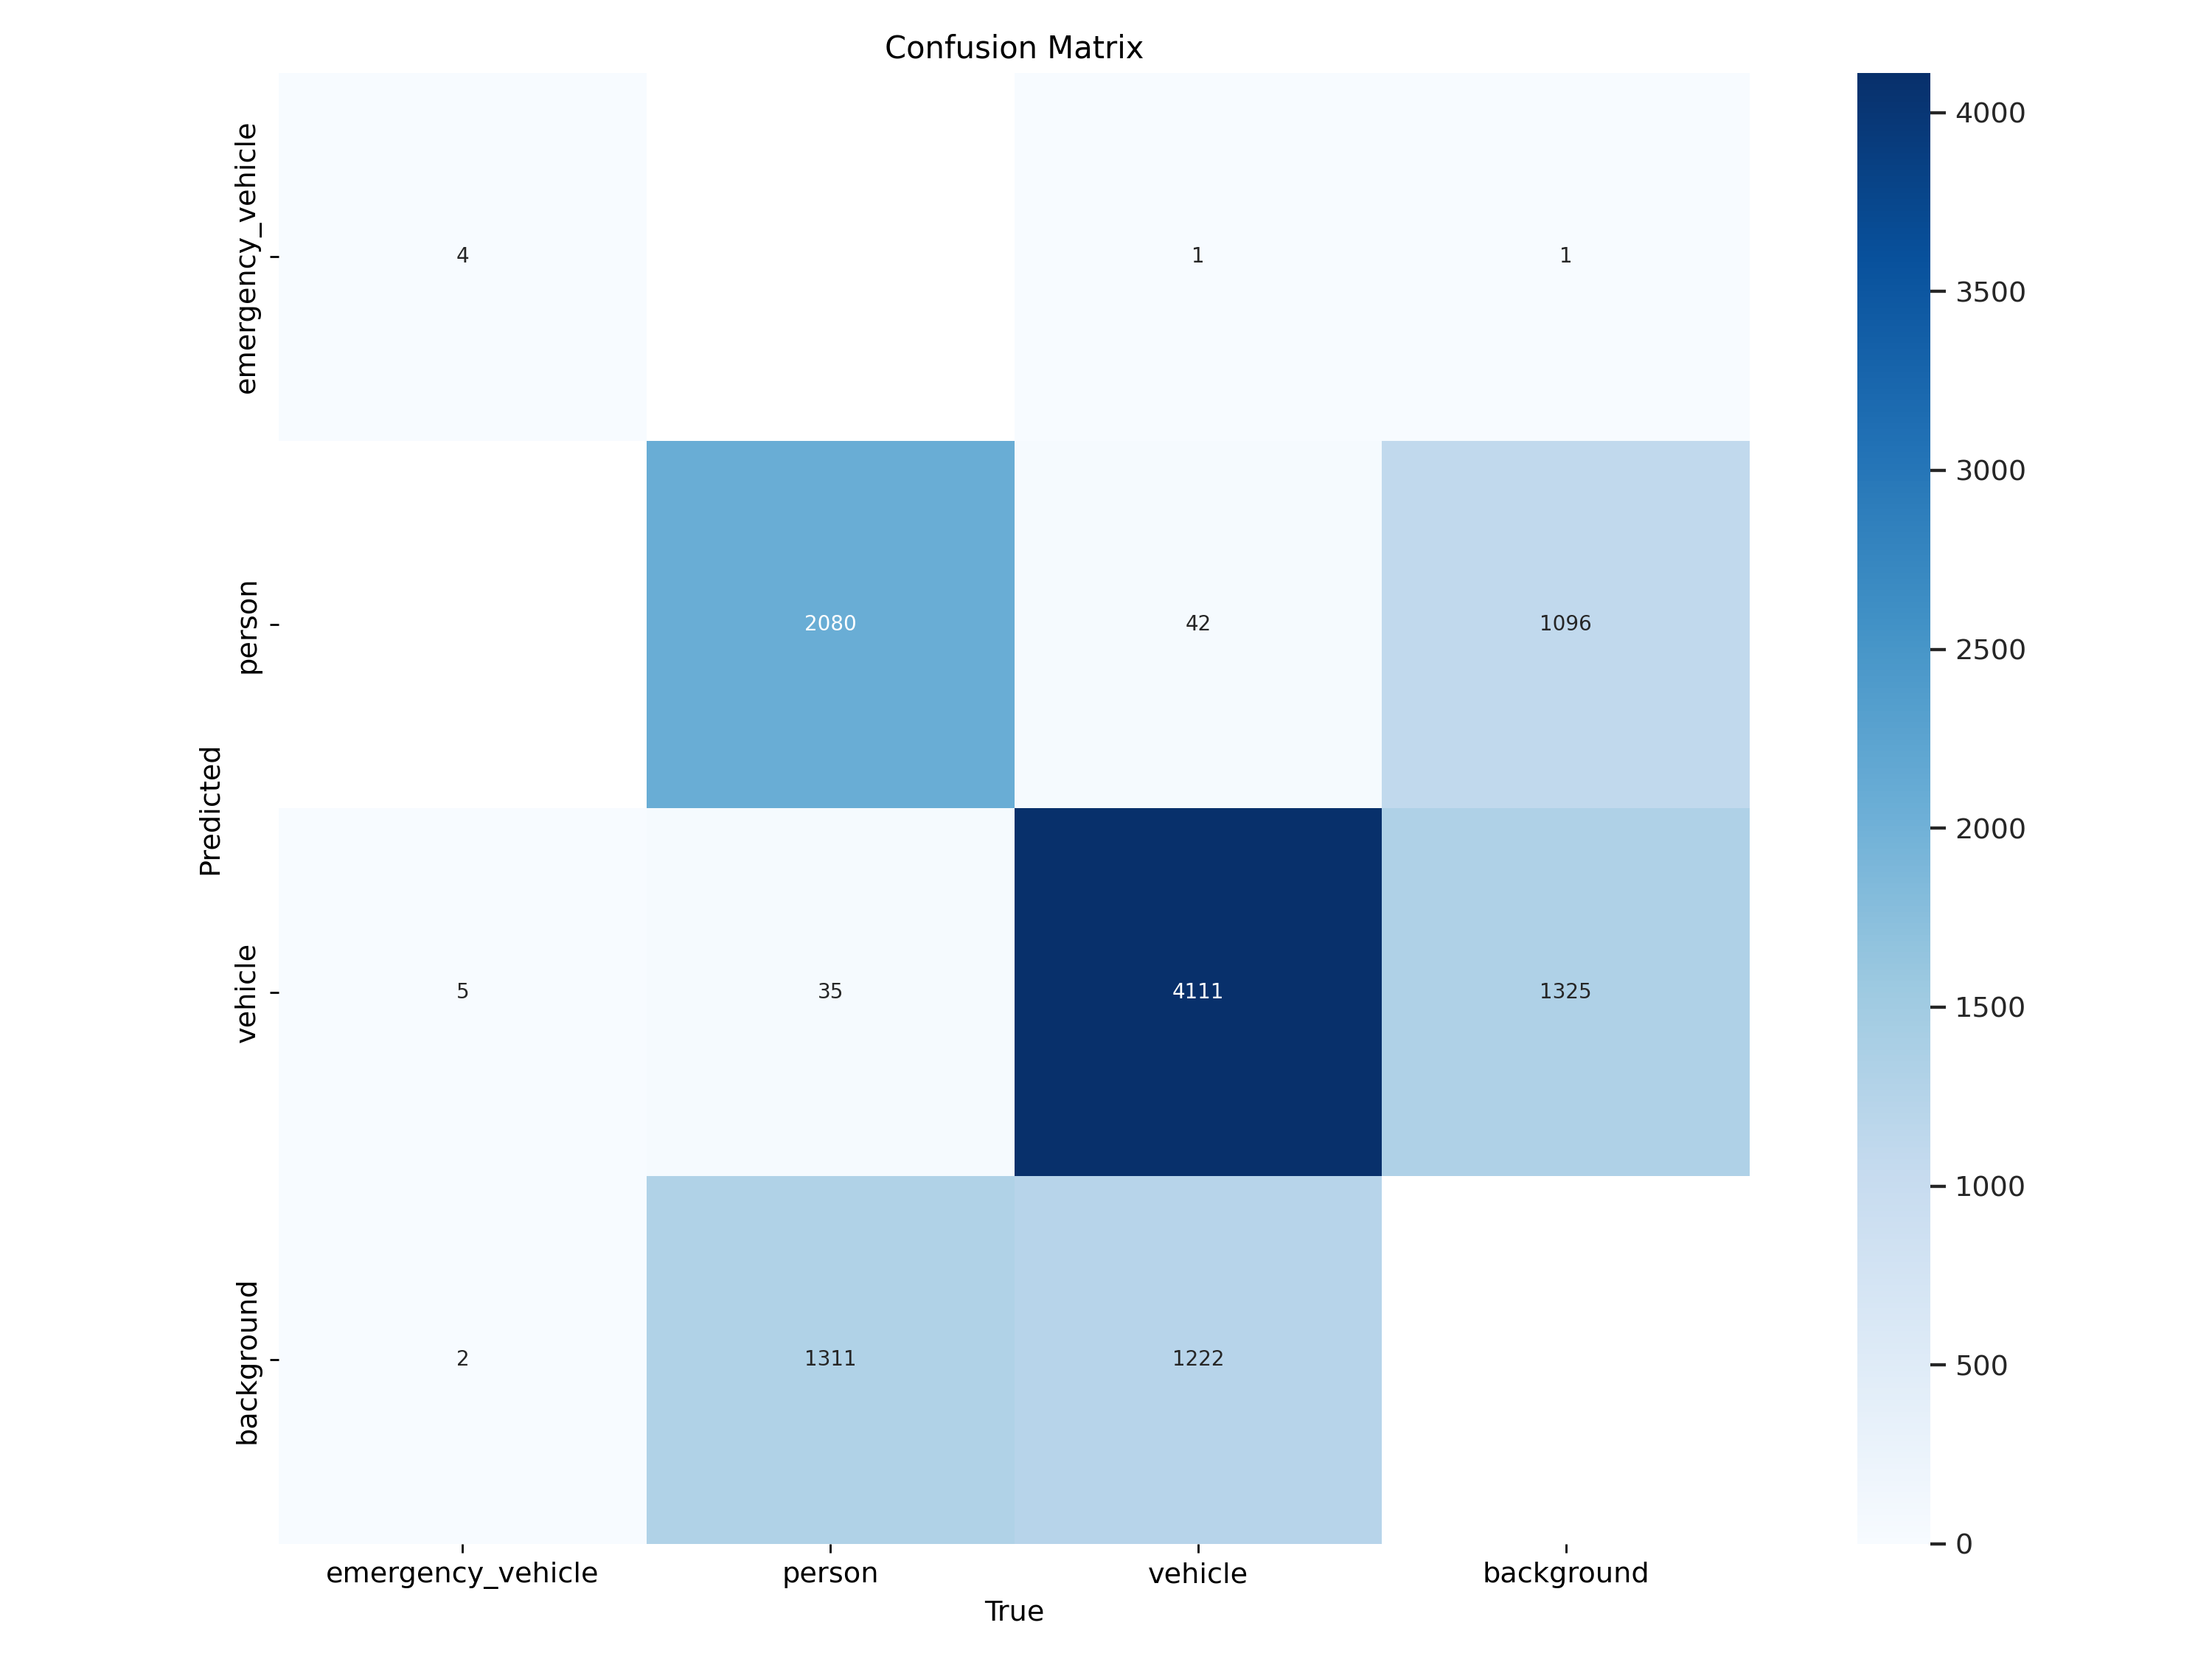
\includegraphics[width=0.9\textwidth]{14.png}
        \caption{Confusion Matrix}
        \label{fig:f7}
    \end{minipage}%
    \hfill % Add some spacing between images
    \vspace{1cm}
    \begin{minipage}{0.5\textwidth}
        \centering
        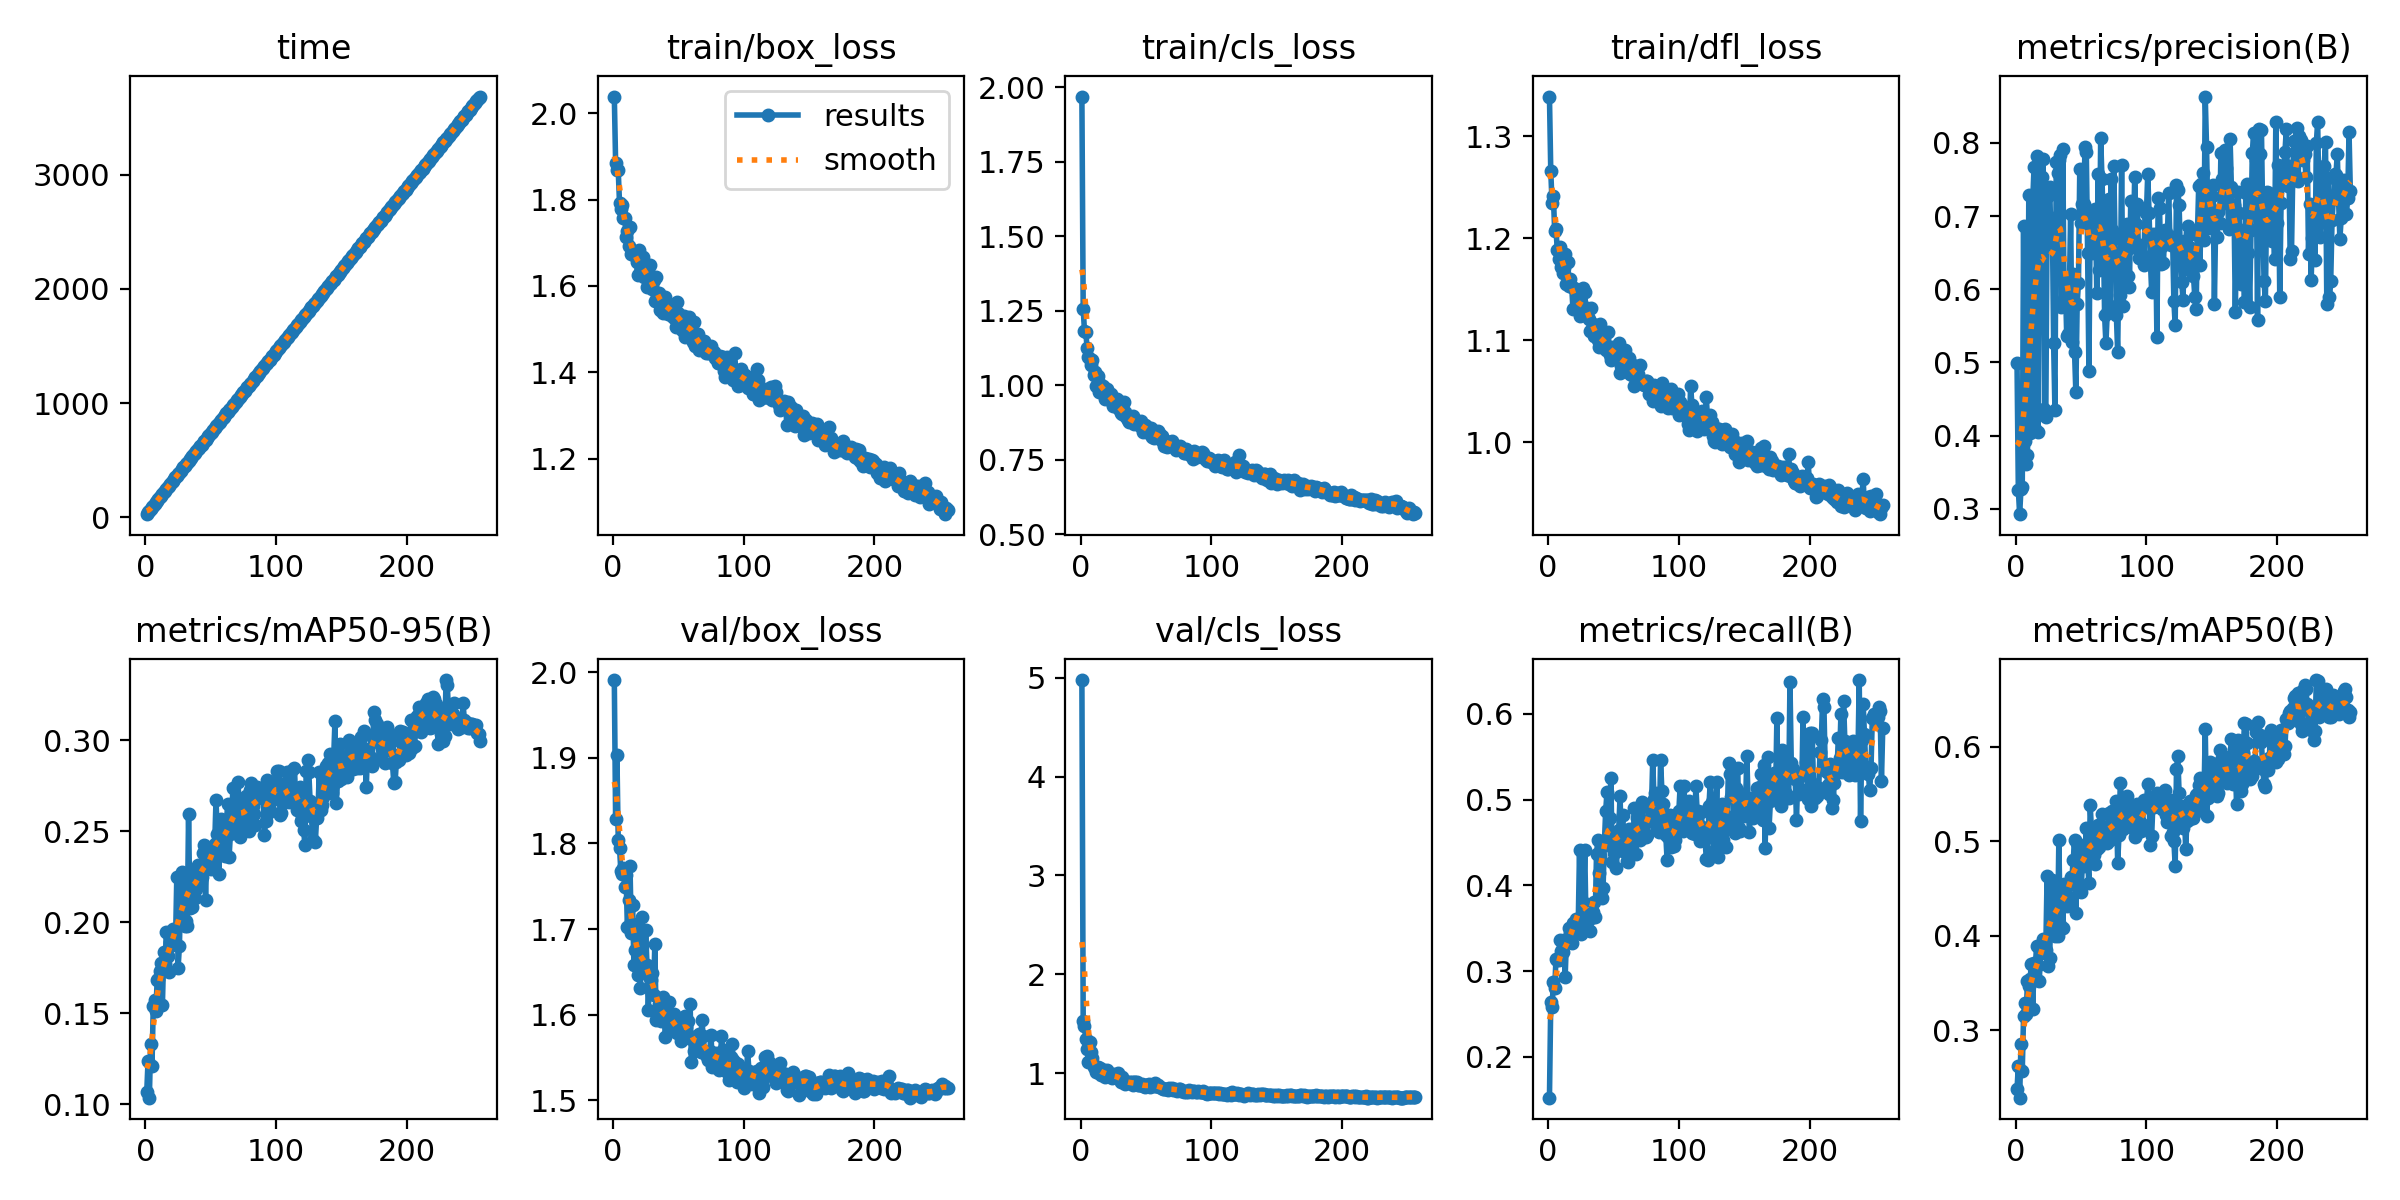
\includegraphics[width=0.9\textwidth]{15.png}
        \caption{Model progression over training epochs.}
        \label{fig:f8}
    \end{minipage}
\end{figure}


\begin{itemize}
    \item \textbf{Class Distribution}:
    \begin{itemize}
        \item The model has detected \textbf{107,004 vehicles}, which account for \textbf{62.5\%} of the total instances. This highlights the model's proficiency in identifying vehicles, which is expected given the prominence of vehicles in traffic scenes.
        \item \textbf{63,541 pedestrians} were detected, making up \textbf{37.1\%} of the total instances. This demonstrates that the model can effectively differentiate between pedestrians and vehicles.
        \item \textbf{781 emergency vehicles} were detected, representing only \textbf{0.5\%} of the total instances. While this is a small portion of the overall traffic, the low proportion reflects the inherent rarity of emergency vehicles in typical traffic datasets(see Fig \ref{fig:f6}).
    \end{itemize}

    \item \textbf{Bounding Box Analysis}:
    \begin{itemize}
        \item The model is highly accurate at identifying vehicles and pedestrians, as shown by the large number of bounding boxes correctly drawn for these categories.
        \item Emergency vehicle detection, while limited in quantity, is crucial. The lower number of emergency vehicles is expected given their scarcity, but improvements can still be made in this area to ensure all emergency vehicles are accurately detected in real-time.
    \end{itemize}

    \item \textbf{Model Accuracy}:
    \begin{itemize}
        \item With an accuracy for the model shows strong potential for practical deployment in real-world traffic management systems (see Table \ref{table:accuracy}). However, there is still room for improvement, especially in fine-tuning the model's sensitivity to emergency vehicles, which are a critical class for priority-based traffic systems.
    \end{itemize}

    \item \textbf{Class Imbalance}:
    \begin{itemize}
        \item The data reflects an inherent imbalance in the dataset, with vehicles being the dominant class, followed by pedestrians. Emergency vehicles, being a rare class, may require special treatment in the training process (e.g., oversampling, data augmentation, or class weighting) to improve detection rates.
    \end{itemize}

\end{itemize}




\begin{table}[H]
    \centering
    \hspace*{-1cm} % Move the table 1 cm to the left
    \setlength{\arrayrulewidth}{0.4pt}
    \renewcommand{\arraystretch}{1.2} % Reduced space between rows for compactness
    \caption{Accuracy, Epochs, and mAP50 with Different Dataset Sizes on YOLOv11}
    \vspace{0.3cm}
    \setlength{\tabcolsep}{4pt}       % Reduce space between columns
    \begin{tabular}{|>{\centering\arraybackslash}m{2.4cm}|c|c|c|c|}
        \hline
        \rowcolor{cyan!20}
        \textbf{Number of images} & \textbf{500} & \textbf{1000} & \textbf{2000} & \textbf{3000} \\ 
        \hline
        \textbf{Vehicles (\%)(max)}       & 83  & 85  & 91  & 94  \\ 
        \hline
        \textbf{Emergency Vehicles (\%)(max)} & 65  & 72  & 83  & 89  \\ 
        \hline
        \textbf{Pedestrians (\%)(max)}    & 63  & 71  & 84  & 89  \\ 
        \hline
        \textbf{Epochs}              & 128, 256 & 128, 256 & 128, 256 & 128, 256 \\ 
        \hline
        \textbf{mAP50 (\%) (max)}    & 67  & 79  & 85  & 91  \\ 
        \hline
        \textbf{Time of training}    & 40 min & 65 min & 110 min & 215 min \\ 
        \hline
    \end{tabular}
    \label{table:accuracy}
\end{table}



 
The system will reduce average vehicle wait times by \textbf{33\%}, optimizing traffic flow through dynamic signal control in Bangladesh \cite{clar:a10}. This is especially important in Dhaka, where average speeds can drop to as low as 4.8 km/h during peak hours\cite{clar:a1}. We hope after implementing the Emergency vehicle response times will reduced significantly. From research, it seems up to \textbf{56\%}  emergency vehicles are delayed due to traffic problems \cite{clar:a11}. So, real-time detection and prioritization of ambulances and fire trucks help people a lot. This improvement is crucial in Dhaka, where traffic congestion delays emergency services, creating life-threatening situations. The system reduced the need for manual human effect, allowing for automated management based on real-time data footage. This minimized human error, ensuring smoother traffic flow, a major advantage given Dhaka’s dependency on traffic police. By implementing starvation management techniques, the system prevented lanes from being blocked or underutilized for long periods, a frequent and hectic issue in Dhaka’s traffic congestion. The system’s use of hardware like Arduino, USB NodeMCU, and Raspberry Pi enabled reliable performance across multiple intersections without significant degradation, supporting its scalability for larger urban areas like Dhaka. The system adapted well to Dhaka’s unpredictable traffic patterns, such as sudden surges in traffic caused by events or road closures, ensuring real-time adjustments to minimize congestion and helping people a lot. The prioritization of emergency vehicles (Ambulance, fire truck, etc) and the reduction in congestion significantly enhanced public safety and daily commuting efficiency, contributing to fewer delays and a smoother flow of traffic, which is critical in a densely populated city like Dhaka and other cities.

\section{Conclusion and Future Work}
Regarding traffic conditions in urban areas, To overcome the issue of traffic congestion we did the proper paperwork. we collected data from many key junctions of Dhaka city. After collecting those data we annotated them in different sections of classification. We achieved almost 91\% accuracy. We also set a goal of preventing starvation on every lane by using an automatic detection system using cameras and also succeded in identifying the emergency vehicles first as a priority demand. Future work will involve enhancing the system’s abilities to include more advanced fateful analytics exploring its integration with smart city initiatives and helping to find a solution after a high time.



\begin{thebibliography}{00}
\bibitem{clar:a1}
Kallol Mustafa, "Why exactly is Dhaka the slowest city in the world?" The Daily Star, Oct. 8, 2023. [Online]. Available: https://www.thedailystar.net/opinion/views/news/why-exactly-dhaka-the-slowest-city-the-world-3436751

\bibitem{clar:a2}
T. J. Karim, "Traffic Gridlock: Time Wasted in Dhaka," Dhaka Tribune, Dec. 5, 2022.

\bibitem{clar:a3}
Y. J. Yao, R. W. Yang, and L. Liu,(2020) "Design of Intelligent Traffic Management System Based on Video Detection Technology," IEEE Access, vol. 8, pp. 67278-67289.

\bibitem{clar:a4}
K. R. K. Singh, P. S. K. Prasad, and M. S. P. K. Roy, "Real-time Traffic Monitoring and Analysis Using YOLOv3 Model," Journal of Intelligent Transportation Systems, vol. 25, no. 5, pp. 509-520, 2021.

\bibitem{clar:a5}
Rahman, M. M., & Mohiuddin, M. (2020). "Traffic Management in Dhaka City: A Critical Review." Journal of Urban Planning and Development, 146(1), 04019029.

\bibitem{clar:a6}
Zhang, D., Wang, Y., & Liu, X. (2020). "Intelligent Traffic Light Control Using Deep Reinforcement Learning with Object Detection." IEEE Transactions on Intelligent Transportation Systems, 20(3), 1-10.

\bibitem{clar:a7}
J. D. J. Wu, M. R. Bell, and M. T. Williams, (2014). "The Effect of Traffic Congestion on Emergency Vehicle Response Times," Journal of Transportation Engineering, vol. 140, no. 8. [Online]. Available: https://ascelibrary.org/doi/abs/10.1061/(ASCE)TE.1943-5436.0000687

\bibitem{clar:a8}
Farooq, M., Habib, M. A., & Iqbal, M. (2020). "Priority-based Traffic Management System for Emergency Vehicles in Urban Areas." International Journal of Computer Applications, 175(20), 45-50.

\bibitem{clar:a9}
Ahmed, K., & Rahman, M. S. (2019). "Urban Traffic Congestion in Dhaka City: An Empirical Study." International Journal of Traffic and Transportation Engineering, 8(2), 19-30. 

\bibitem{clar:a10}
 Deccan Herald, Mar. 12, 2023. "AI-powered signals in Bengaluru reduce travel time by 33\%". [Online]. Available: https://shorturl.at/EEUsQ

\bibitem{clar:a11}
MM Hossain & A Kroeger. (2017). "87 Transport, delay to care and patient experience in pre-clinical emergency systems in dhaka city, bangladesh: a mixed methods study". [Online]. Available: https://shorturl.at/CpxTO

\bibitem{clar:a12}
N. Sharma, A. Garg, and P. Jain, (2021) "Smart traffic light control system using Raspberry Pi and IoT," International Journal of Computer Science and Network Security, vol. 21, no. 3, pp. 158-164.

\bibitem{clar:a13}
M. S. Islam, S. A. Chowdhury, and M. A. Hossain, (2020) "Design and implementation of an intelligent traffic control system using Arduino and machine learning," International Journal of Intelligent Systems and Applications, vol. 12, no. 4, pp. 42-50.

\bibitem{clar:a14}
J. Redmon, S. Divvala, R. Girshick, and A. Farhadi,(2016). "You Only Look Once: Unified, real-time object detection," Proceedings of the IEEE Conference on Computer Vision and Pattern Recognition (CVPR), pp. 779-788.

\bibitem{clar:a15}
C. Huang, Q. Liu, and D. Zhang,(2019). "YOLO-based traffic signal control system using deep reinforcement learning," Transportation Research Part C: Emerging Technologies, vol. 105, pp. 159-174.

\bibitem{clar:a16}
A. A. Gupta and S. R. Singh, (2020). "Impact of traffic congestion on emergency services in urban areas," International Journal of Transportation Science and Technology, vol. 10, no. 2, pp. 123-135.
\end{thebibliography}


\end{document}
